\chapter{Atoms and Molecules}\label{ch:g7:atoms-and-molecules}

Take a drop of water and cut it in two. Each half is still water. Cut a
half in two again, and again, and again. Could you go on for ever, or
would you reach a piece so small that cutting it once more gives
something that is no longer water at all? Around 400~BC, the Greek
thinker Democritus guessed the answer: matter is made of tiny pieces
that cannot be cut, which he called \emph{\omterm{def:g7:atoms-and-molecules:atom}{atoms}}, from the Greek for
``uncuttable''. It took more than two thousand years, and the work of
the chemists of the nineteenth century, to turn that guess into
science. This chapter describes the pieces --- \omterm{def:g7:atoms-and-molecules:atom}{atoms} --- and how they
group into \omterm{def:g7:atoms-and-molecules:molecule}{molecules}.

\begin{recall}
A \omterm{def:g6:pure-substances-and-mixtures:pure-substance}{pure substance}, such as water or oxygen, is made of one single
\omterm{def:g6:pure-substances-and-mixtures:species}{chemical species}; a \omterm{def:g6:pure-substances-and-mixtures:mixture}{mixture}, such as \omterm{def:g4:air-a-mixture-of-gases:air}{air}, contains several
(\cref{ch:g6:pure-substances-and-mixtures}). \omterm{def:g4:air-a-mixture-of-gases:air}{Air} is about four fifths
nitrogen and one fifth oxygen (\cref{ch:g4:air-a-mixture-of-gases}).
\end{recall}

\section{Atoms}

\begin{definition}[Atom]\label{def:g7:atoms-and-molecules:atom}
All matter is built from extremely small particles called
\emph{atoms}\index{atom}. There are only about a hundred different
kinds of atoms in nature, and every substance --- water, \omterm{def:g4:air-a-mixture-of-gases:air}{air}, iron,
sugar, our own bodies --- is made of atoms of a few of these kinds.
\end{definition}

\begin{proposition}[Atoms are tiny]\label{prop:g7:atoms-and-molecules:tiny}
% ledger: const:a0, earth:diameter (8 cm apple: 12756 km / 8 cm = 1.6 x 10^8;
% 0.1-0.15 nm x 1.6 x 10^8 = 1.7-2.4 cm, a small cherry)
The smallest \omterm{def:g7:atoms-and-molecules:atom}{atom}, the hydrogen \omterm{def:g7:atoms-and-molecules:atom}{atom}, measures about a ten-millionth of
a millimetre across; the others are at most a few times larger. Ten
million hydrogen \omterm{def:g7:atoms-and-molecules:atom}{atoms} in a row would make a line one millimetre long.
To picture it: if an apple were blown up to the size of the Earth, each
of its \omterm{def:g7:atoms-and-molecules:atom}{atoms} would be about the size of a small cherry.
\end{proposition}

\begin{remark}[Seen without being seen]\label{rem:g7:atoms-and-molecules:seen}
No microscope using light can show an \omterm{def:g7:atoms-and-molecules:atom}{atom}: \omterm{def:g7:atoms-and-molecules:atom}{atoms} are far smaller than
the waves of light. Since the 1980s, special microscopes that feel a
surface with an extremely fine tip have made images in which single
\omterm{def:g7:atoms-and-molecules:atom}{atoms} appear as bumps.
\end{remark}

\begin{definition}[Symbol of an atom]\label{def:g7:atoms-and-molecules:symbol}
Each kind of \omterm{def:g7:atoms-and-molecules:atom}{atom} has a name and a \emph{symbol}\index{symbol of an atom}:
one capital letter, sometimes followed by one small letter. The
symbol is the same in every language.
\end{definition}

\begin{center}
\small
\begin{tabular}{llll|llll}
\hline
\omterm{def:g7:atoms-and-molecules:atom}{atom} & \omterm{def:g7:atoms-and-molecules:symbol}{symbol} & & model colour & \omterm{def:g7:atoms-and-molecules:atom}{atom} & \omterm{def:g7:atoms-and-molecules:symbol}{symbol} & & model colour \\
\hline
hydrogen & \ce{H} & \tikz\node[aH]{}; & white & sodium & \ce{Na} & \tikz\node[aNa]{}; & purple \\
carbon & \ce{C} & \tikz\node[aC]{}; & black & sulfur & \ce{S} & \tikz\node[aS]{}; & yellow \\
nitrogen & \ce{N} & \tikz\node[aN]{}; & blue & chlorine & \ce{Cl} & \tikz\node[aCl]{}; & green \\
oxygen & \ce{O} & \tikz\node[aO]{}; & red & iron, copper & \ce{Fe}, \ce{Cu} & & --- \\
\hline
\end{tabular}
\end{center}

\begin{remark}[Where symbols come from]\label{rem:g7:atoms-and-molecules:latin}
Most \omterm{def:g7:atoms-and-molecules:symbol}{symbols} are the first letters of the name: \ce{H} for hydrogen,
\ce{C} for carbon, \ce{O} for oxygen. Some come from an older, Latin
name: \ce{Na} for sodium (\emph{natrium}), \ce{Fe} for iron
(\emph{ferrum}), \ce{Cu} for copper (\emph{cuprum}). The second letter
is always small: \ce{Co} is the cobalt \omterm{def:g7:atoms-and-molecules:atom}{atom}, while CO, with a capital
O, is something else entirely.
\end{remark}

\begin{history}[Dalton's atoms, 1808]
In 1808 the chemist John Dalton published a table of the \omterm{def:g7:atoms-and-molecules:atom}{atoms}
then known, each drawn as a small circle with its own sign. He was the
first to say that every \omterm{def:g7:atoms-and-molecules:atom}{atom} of one kind has the same weight, and that
chemists could compare these weights. But he also guessed that water was
one hydrogen \omterm{def:g7:atoms-and-molecules:atom}{atom} joined to one oxygen \omterm{def:g7:atoms-and-molecules:atom}{atom}; it took another fifty
years for chemists to agree that a water \omterm{def:g7:atoms-and-molecules:molecule}{molecule} holds \emph{two}
hydrogen \omterm{def:g7:atoms-and-molecules:atom}{atoms}.
\end{history}

\begin{omfigure}
\begin{minipage}[b]{0.3\linewidth}\centering
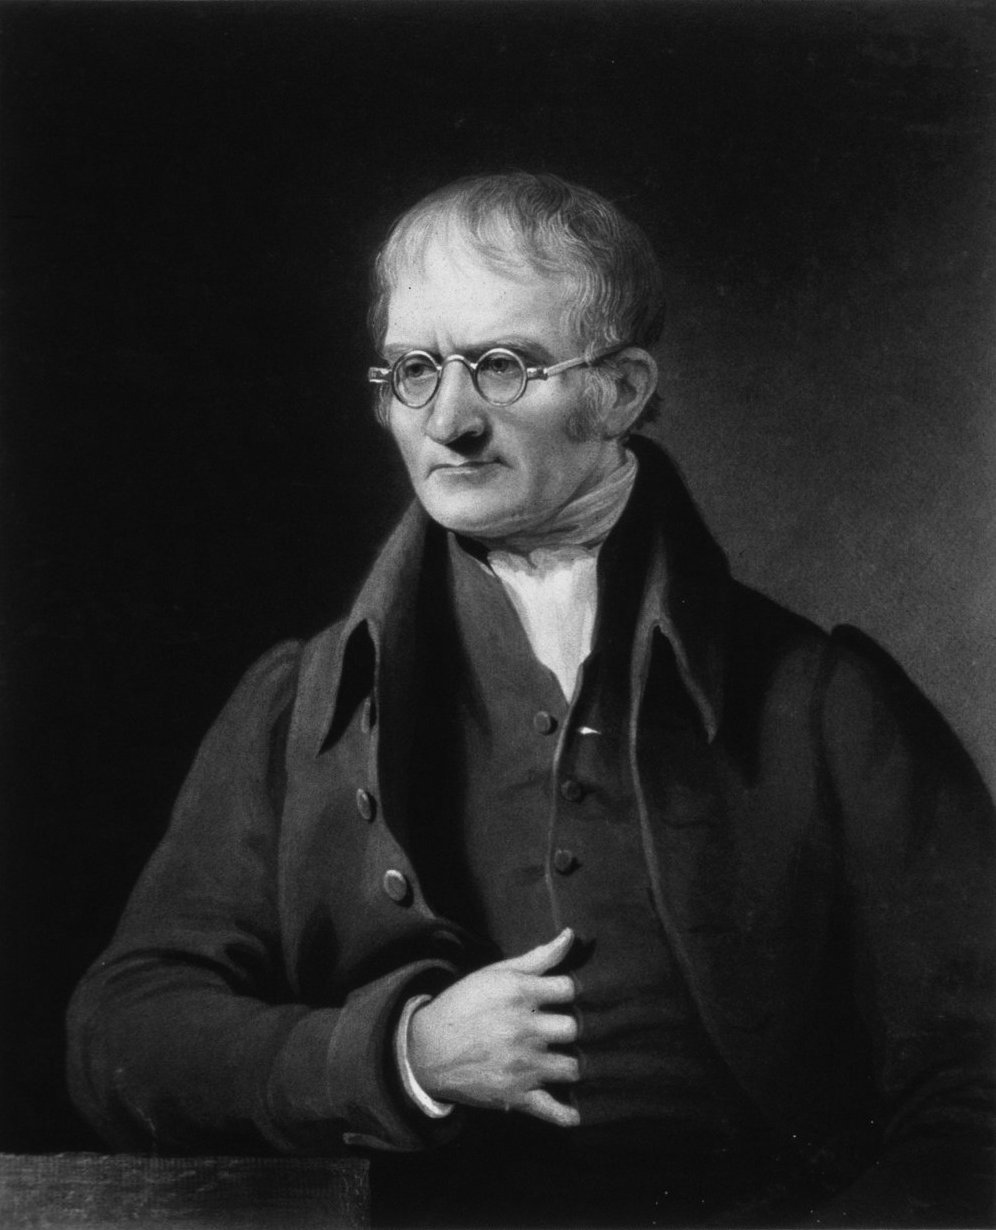
\includegraphics[width=\linewidth]{images/book1/dalton.jpg}

{\small John Dalton (1766--1844).}
\end{minipage}\hfill
\begin{minipage}[b]{0.66\linewidth}\centering
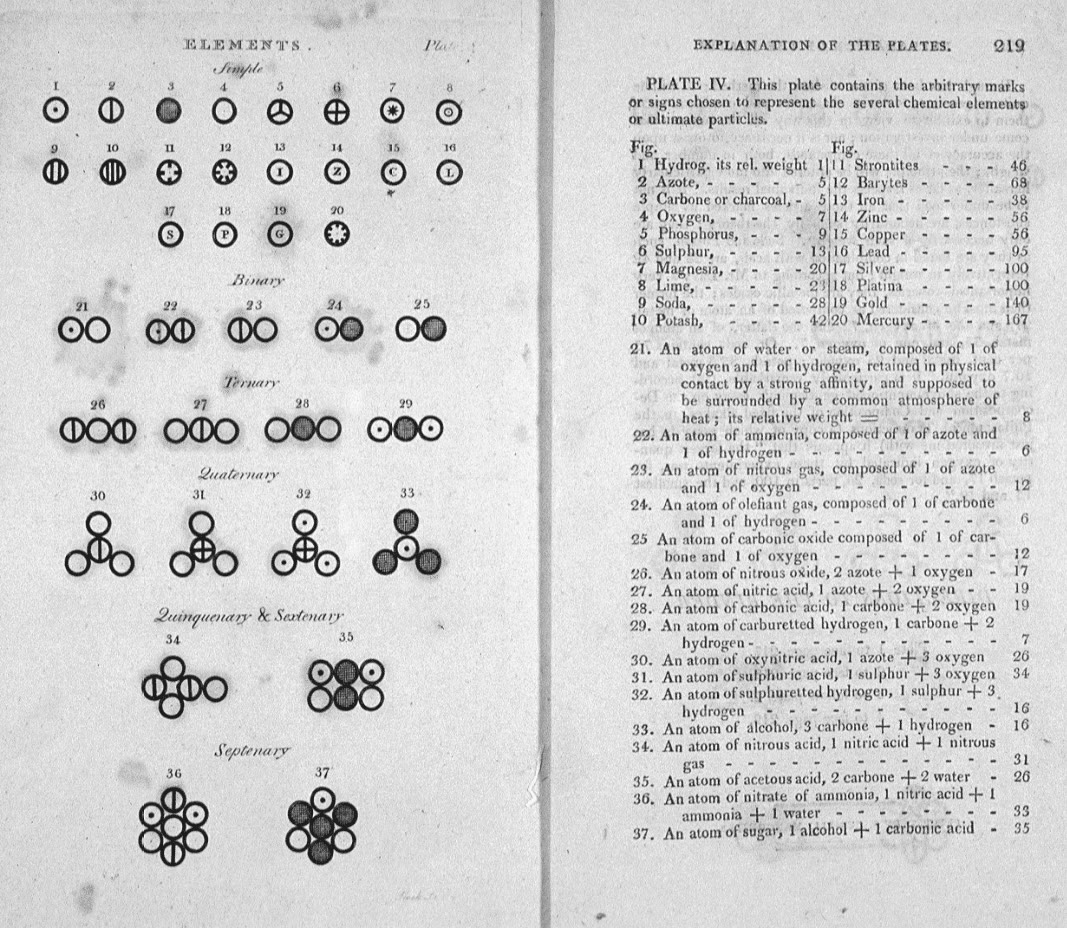
\includegraphics[width=\linewidth]{images/book1/dalton-symbols.jpg}

{\small Dalton's table of 1808: his water, sign 21, is one circle of
hydrogen beside one of oxygen.}
\end{minipage}
\end{omfigure}

\section{Molecules}

\begin{definition}[Molecule]\label{def:g7:atoms-and-molecules:molecule}
A \emph{molecule}\index{molecule} is a group of \omterm{def:g7:atoms-and-molecules:atom}{atoms} held tightly
together. A molecule is the smallest piece of a substance that is
still that substance: a water molecule is the smallest possible amount
of water.
\end{definition}

\begin{example}[Seven molecules]\label{ex:g7:atoms-and-molecules:seven}
\begin{itemize}
  \item the \emph{hydrogen} \omterm{def:g7:atoms-and-molecules:molecule}{molecule}: two hydrogen \omterm{def:g7:atoms-and-molecules:atom}{atoms};
  \item the \emph{oxygen} \omterm{def:g7:atoms-and-molecules:molecule}{molecule}, which we breathe: two oxygen \omterm{def:g7:atoms-and-molecules:atom}{atoms};
  \item the \emph{nitrogen} \omterm{def:g7:atoms-and-molecules:molecule}{molecule}, four fifths of the \omterm{def:g4:air-a-mixture-of-gases:air}{air}: two
        nitrogen \omterm{def:g7:atoms-and-molecules:atom}{atoms};
  \item the \emph{water} \omterm{def:g7:atoms-and-molecules:molecule}{molecule}: two hydrogen \omterm{def:g7:atoms-and-molecules:atom}{atoms} and one oxygen
        \omterm{def:g7:atoms-and-molecules:atom}{atom};
  \item the \emph{carbon dioxide} \omterm{def:g7:atoms-and-molecules:molecule}{molecule}, which we breathe out: one
        carbon \omterm{def:g7:atoms-and-molecules:atom}{atom} and two oxygen \omterm{def:g7:atoms-and-molecules:atom}{atoms};
  \item the \emph{methane} \omterm{def:g7:atoms-and-molecules:molecule}{molecule}, the main part of the natural gas
        burnt in gas cookers: one carbon \omterm{def:g7:atoms-and-molecules:atom}{atom} and four hydrogen \omterm{def:g7:atoms-and-molecules:atom}{atoms};
  \item the \emph{nitrous oxide} \omterm{def:g7:atoms-and-molecules:molecule}{molecule}, an anaesthetic gas: two
        nitrogen \omterm{def:g7:atoms-and-molecules:atom}{atoms} and one oxygen \omterm{def:g7:atoms-and-molecules:atom}{atom}.
\end{itemize}
\end{example}

\begin{omfigure}
\begin{tikzpicture}[font=\small]
  % hydrogen
  \begin{scope}[xshift=0cm]
    \node[aH] (a) at (-0.25,0) {}; \node[aH] (b) at (0.25,0) {};
    \begin{scope}[on background layer]\draw[bond] (a.center) -- (b.center);\end{scope}
    \node at (0,-1.05) {hydrogen};
  \end{scope}
  % oxygen
  \begin{scope}[xshift=2.6cm]
    \node[aO] (a) at (-0.33,0) {}; \node[aO] (b) at (0.33,0) {};
    \begin{scope}[on background layer]
      \draw[bond, line width=1.1pt] ([yshift=1.6pt]a.center) -- ([yshift=1.6pt]b.center);
      \draw[bond, line width=1.1pt] ([yshift=-1.6pt]a.center) -- ([yshift=-1.6pt]b.center);
    \end{scope}
    \node at (0,-1.05) {oxygen};
  \end{scope}
  % nitrogen
  \begin{scope}[xshift=5.2cm]
    \node[aN] (a) at (-0.33,0) {}; \node[aN] (b) at (0.33,0) {};
    \begin{scope}[on background layer]
      \foreach \d in {-2.4,0,2.4}
        \draw[bond, line width=0.9pt] ([yshift=\d pt]a.center) -- ([yshift=\d pt]b.center);
    \end{scope}
    \node at (0,-1.05) {nitrogen};
  \end{scope}
  % water
  \begin{scope}[xshift=7.8cm, yshift=0.2cm]
    \node[aO] (o) at (0,0) {};
    \node[aH] (h1) at (-0.62,-0.48) {}; \node[aH] (h2) at (0.62,-0.48) {};
    \begin{scope}[on background layer]
      \draw[bond] (o.center) -- (h1.center); \draw[bond] (o.center) -- (h2.center);
    \end{scope}
    \node at (0,-1.25) {water};
  \end{scope}
  % carbon dioxide
  \begin{scope}[xshift=0.9cm, yshift=-2.7cm]
    \node[aO] (a) at (-0.85,0) {}; \node[aC] (c) at (0,0) {}; \node[aO] (b) at (0.85,0) {};
    \begin{scope}[on background layer]
      \foreach \d in {-1.6,1.6} {
        \draw[bond, line width=1.1pt] ([yshift=\d pt]a.center) -- ([yshift=\d pt]c.center);
        \draw[bond, line width=1.1pt] ([yshift=\d pt]c.center) -- ([yshift=\d pt]b.center);}
    \end{scope}
    \node at (0,-1.05) {carbon dioxide};
  \end{scope}
  % methane
  \begin{scope}[xshift=4.4cm, yshift=-2.6cm]
    \node[aC] (c) at (0,0) {};
    \node[aH] (h1) at (0,0.78) {};
    \node[aH] (h2) at (-0.74,-0.3) {};
    \node[aH] (h3) at (0.74,-0.3) {};
    \begin{scope}[on background layer]
      \draw[bond] (c.center) -- (h1.center); \draw[bond] (c.center) -- (h2.center);
      \draw[bond] (c.center) -- (h3.center);
    \end{scope}
    \draw[bond] (c.center) -- (0.22,-0.52);
    \node[aH] at (0.24,-0.58) {};
    \node at (0,-1.15) {methane};
  \end{scope}
  % nitrous oxide
  \begin{scope}[xshift=7.8cm, yshift=-2.7cm]
    \node[aN] (a) at (-0.8,0) {}; \node[aN] (b) at (0,0) {}; \node[aO] (c) at (0.8,0) {};
    \begin{scope}[on background layer]
      \foreach \d in {-1.6,1.6} {
        \draw[bond, line width=1.1pt] ([yshift=\d pt]a.center) -- ([yshift=\d pt]b.center);
        \draw[bond, line width=1.1pt] ([yshift=\d pt]b.center) -- ([yshift=\d pt]c.center);}
    \end{scope}
    \node at (0,-1.05) {nitrous oxide};
  \end{scope}
\end{tikzpicture}

{\small Ball-and-stick models of the seven \omterm{def:g7:atoms-and-molecules:molecule}{molecules} of
\cref{ex:g7:atoms-and-molecules:seven}. Each stick stands for a bond
between two \omterm{def:g7:atoms-and-molecules:atom}{atoms}; why some \omterm{def:g7:atoms-and-molecules:atom}{atoms} share two or three sticks is
explained in a later chapter.}
\end{omfigure}

\begin{proposition}[Molecules of a pure substance and of a mixture]\label{prop:g7:atoms-and-molecules:pure}
In a \omterm{def:g6:pure-substances-and-mixtures:pure-substance}{pure substance} made of \omterm{def:g7:atoms-and-molecules:molecule}{molecules}, all the \omterm{def:g7:atoms-and-molecules:molecule}{molecules} are identical:
pure water contains only water \omterm{def:g7:atoms-and-molecules:molecule}{molecules}. A \omterm{def:g6:pure-substances-and-mixtures:mixture}{mixture} contains \omterm{def:g7:atoms-and-molecules:molecule}{molecules}
of several kinds: \omterm{def:g4:air-a-mixture-of-gases:air}{air} is mostly nitrogen \omterm{def:g7:atoms-and-molecules:molecule}{molecules} and oxygen
\omterm{def:g7:atoms-and-molecules:molecule}{molecules}, about four of nitrogen for each one of oxygen, with a few
argon \omterm{def:g7:atoms-and-molecules:atom}{atoms} that stay single, and very few \omterm{def:g7:atoms-and-molecules:molecule}{molecules} of carbon dioxide.
\end{proposition}

\begin{omfigure}
\begin{tikzpicture}[font=\small,
    sN/.style={aN, minimum size=3.0mm}, sO/.style={aO, minimum size=2.9mm},
    sH/.style={aH, minimum size=2.1mm}, sAr/.style={om atom, ball color=cyan!60, minimum size=3.4mm}]
  % air
  \draw[omGlass, line width=0.6pt] (0,0) rectangle (3.4,3.4);
  \foreach \x/\y/\r in {0.5/0.6/20, 1.6/0.4/-30, 2.8/0.7/75, 0.6/1.7/110,
                        2.0/1.5/10, 2.9/2.0/-60, 0.9/2.8/40, 2.1/2.9/-15}
    \node[sN] at ($(\x,\y)+(\r:0.12)$) {} node[sN] at ($(\x,\y)+(\r+180:0.12)$) {};
  \foreach \x/\y/\r in {1.3/1.1/60, 1.6/2.3/-40}
    \node[sO] at ($(\x,\y)+(\r:0.12)$) {} node[sO] at ($(\x,\y)+(\r+180:0.12)$) {};
  \node[sAr] at (2.9,3.0) {};
  \node[anchor=north] at (1.7,-0.1) {\textbf{air}: a mixture};
  % water
  \begin{scope}[xshift=5.2cm]
    \draw[omGlass, line width=0.6pt] (0,0) rectangle (3.4,3.4);
    \foreach \x in {0,1,2,3,4} \foreach \y in {0,1,2,3,4} {
      \pgfmathsetmacro{\ang}{mod(73*\x+41*\y,360)}
      \begin{scope}[shift={({0.36+0.67*\x},{0.4+0.66*\y})}, rotate=\ang]
        \node[sH] at (-0.16,-0.12) {}; \node[sH] at (0.16,-0.12) {};
        \node[sO] at (0,0) {};
      \end{scope}}
    \node[anchor=north] at (1.7,-0.1) {\textbf{water}: a pure substance};
  \end{scope}
\end{tikzpicture}

{\small Zooming in, enormously. Left: in \omterm{def:g4:air-a-mixture-of-gases:air}{air}, \omterm{def:g7:atoms-and-molecules:molecule}{molecules} of nitrogen
(blue) far outnumber those of oxygen (red), and an argon \omterm{def:g7:atoms-and-molecules:atom}{atom} (pale
blue) travels alone; the \omterm{def:g7:atoms-and-molecules:molecule}{molecules} of a gas are far apart. Right: in
liquid water, the \omterm{def:g7:atoms-and-molecules:molecule}{molecules} are all identical and touch one another.}
\end{omfigure}

\section{Chemical formulas}

\begin{definition}[Chemical formula]\label{def:g7:atoms-and-molecules:formula}
The \emph{chemical formula}\index{chemical formula} of a \omterm{def:g7:atoms-and-molecules:molecule}{molecule} lists
the \omterm{def:g7:atoms-and-molecules:symbol}{symbols} of its \omterm{def:g7:atoms-and-molecules:atom}{atoms}, each followed by a small number written
below the line --- the \emph{subscript}\index{subscript} --- giving how many \omterm{def:g7:atoms-and-molecules:atom}{atoms} of
that kind the \omterm{def:g7:atoms-and-molecules:molecule}{molecule} contains. A subscript 1 is not written.
\end{definition}

\begin{example}[The seven formulas]\label{ex:g7:atoms-and-molecules:formulas}
The \omterm{def:g7:atoms-and-molecules:molecule}{molecules} of \cref{ex:g7:atoms-and-molecules:seven} have these
formulas:
\begin{center}
\begin{tabular}{lcl}
\hline
\omterm{def:g7:atoms-and-molecules:molecule}{molecule} & formula & \omterm{def:g7:atoms-and-molecules:atom}{atoms} \\
\hline
hydrogen & \ce{H2} & 2 hydrogen \\
oxygen & \ce{O2} & 2 oxygen \\
nitrogen & \ce{N2} & 2 nitrogen \\
water & \ce{H2O} & 2 hydrogen, 1 oxygen \\
carbon dioxide & \ce{CO2} & 1 carbon, 2 oxygen \\
methane & \ce{CH4} & 1 carbon, 4 hydrogen \\
nitrous oxide & \ce{N2O} & 2 nitrogen, 1 oxygen \\
\hline
\end{tabular}
\end{center}
\end{example}

\begin{method}[Reading a formula]\label{met:g7:atoms-and-molecules:read}
To read the formula of a \omterm{def:g7:atoms-and-molecules:molecule}{molecule}:
\begin{enumerate}
  \item split it into \omterm{def:g7:atoms-and-molecules:symbol}{symbols}: each one starts with a capital letter;
  \item after each \omterm{def:g7:atoms-and-molecules:symbol}{symbol}, read the \omterm{def:g7:atoms-and-molecules:formula}{subscript} (no \omterm{def:g7:atoms-and-molecules:formula}{subscript} means 1);
  \item add up the \omterm{def:g7:atoms-and-molecules:formula}{subscripts} to get the total number of \omterm{def:g7:atoms-and-molecules:atom}{atoms}.
\end{enumerate}
For \ce{C2H6O} (ethanol, the alcohol of drinks): 2 carbon, 6 hydrogen,
1 oxygen, 9 \omterm{def:g7:atoms-and-molecules:atom}{atoms} in all.
\end{method}

\begin{remark}[A number in front]\label{rem:g7:atoms-and-molecules:coefficient}
A number written in front of a formula counts \omterm{def:g7:atoms-and-molecules:molecule}{molecules}: \ce{3H2O} means
three water \omterm{def:g7:atoms-and-molecules:molecule}{molecules}, which together hold 6 hydrogen \omterm{def:g7:atoms-and-molecules:atom}{atoms} and 3 oxygen
\omterm{def:g7:atoms-and-molecules:atom}{atoms}. Do not confuse \ce{O2}, one \omterm{def:g7:atoms-and-molecules:molecule}{molecule} made of two oxygen \omterm{def:g7:atoms-and-molecules:atom}{atoms},
with \ce{2O}, two oxygen \omterm{def:g7:atoms-and-molecules:atom}{atoms} that are not joined.
\end{remark}

\begin{example}[Methane in the kitchen]\label{ex:g7:atoms-and-molecules:methane}
The natural gas of a gas cooker is mostly methane, \ce{CH4}. Each of its
\omterm{def:g7:atoms-and-molecules:molecule}{molecules} is one carbon \omterm{def:g7:atoms-and-molecules:atom}{atom} with four hydrogen \omterm{def:g7:atoms-and-molecules:atom}{atoms} around it. The gas
is invisible and has no smell: the smell of ``gas'' is a substance added
on purpose, so that a leak is noticed.
\end{example}

\begin{omfigure}
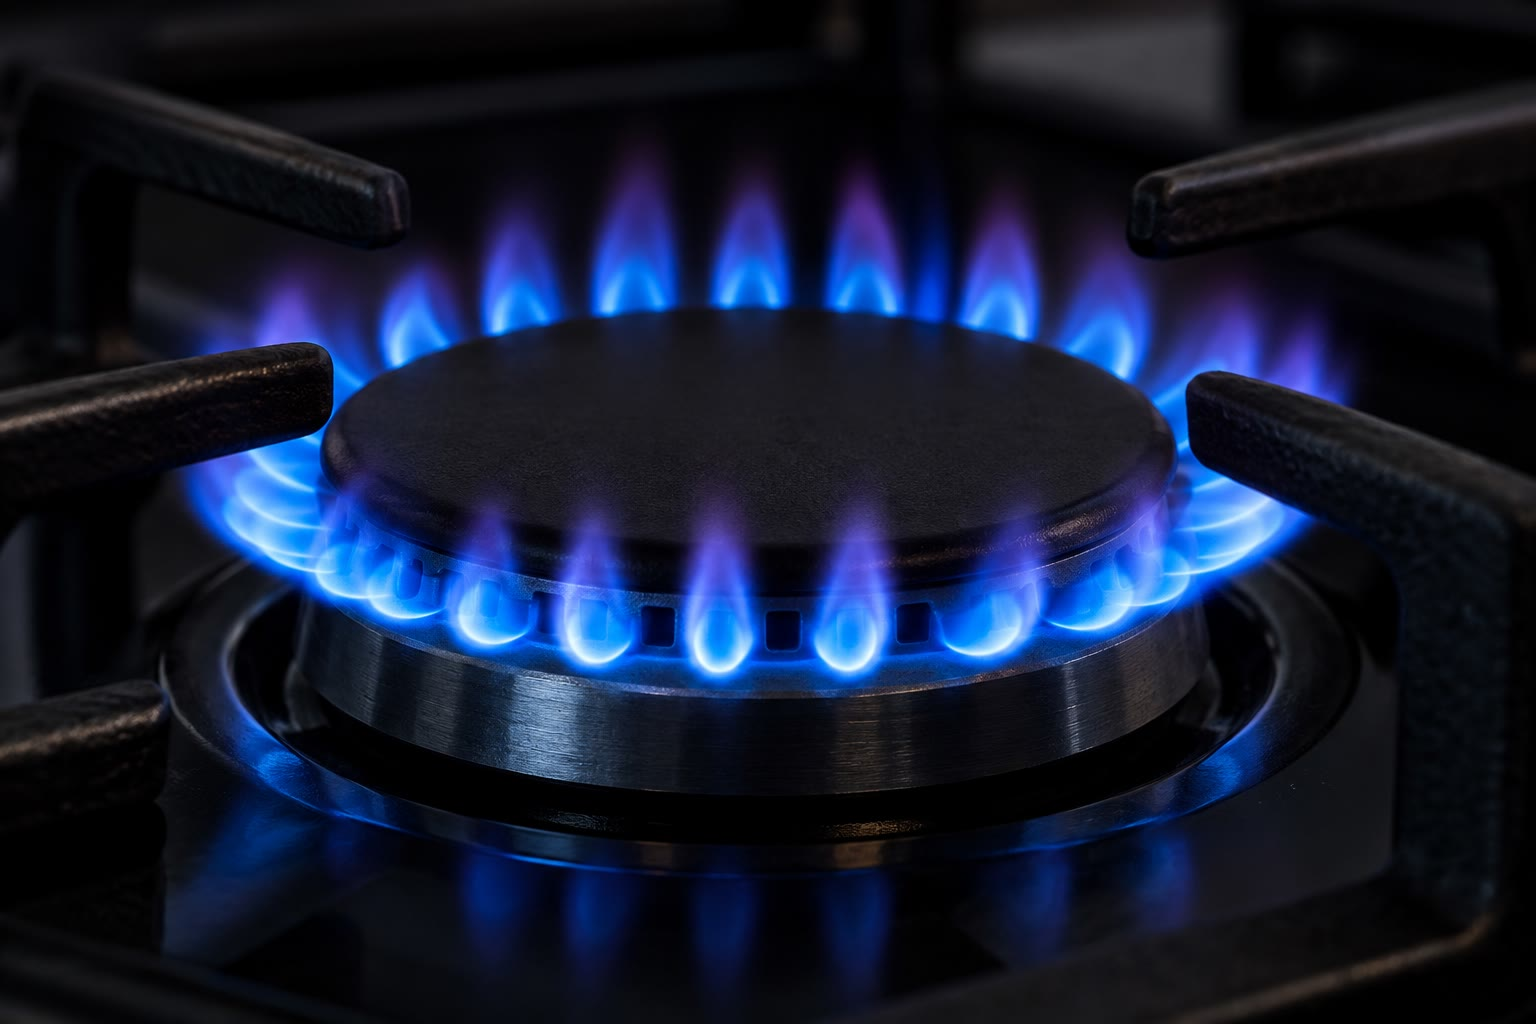
\includegraphics[width=0.5\linewidth]{images/book1/ai/g7-gas-flame.jpg}

{\small The blue flame of a gas cooker: the methane of natural gas is \omterm{def:g4:what-a-fire-needs:burning}{burning}.}
\end{omfigure}

\section{Molecular models}

\begin{remark}[Models, and their colours]\label{rem:g7:atoms-and-molecules:models}
Chemists build \emph{molecular models} with balls for the \omterm{def:g7:atoms-and-molecules:atom}{atoms} and
sticks for the bonds between them. The colours are a convention used all
over the world --- carbon black, hydrogen white, oxygen red, nitrogen
blue --- and not the real colour of \omterm{def:g7:atoms-and-molecules:atom}{atoms}: a single \omterm{def:g7:atoms-and-molecules:atom}{atom} has no colour
at all. A model also shows the shape of a \omterm{def:g7:atoms-and-molecules:molecule}{molecule}, which a formula does
not: the water \omterm{def:g7:atoms-and-molecules:molecule}{molecule} is bent, the carbon dioxide \omterm{def:g7:atoms-and-molecules:molecule}{molecule} is
straight.
\end{remark}

\begin{omfigure}
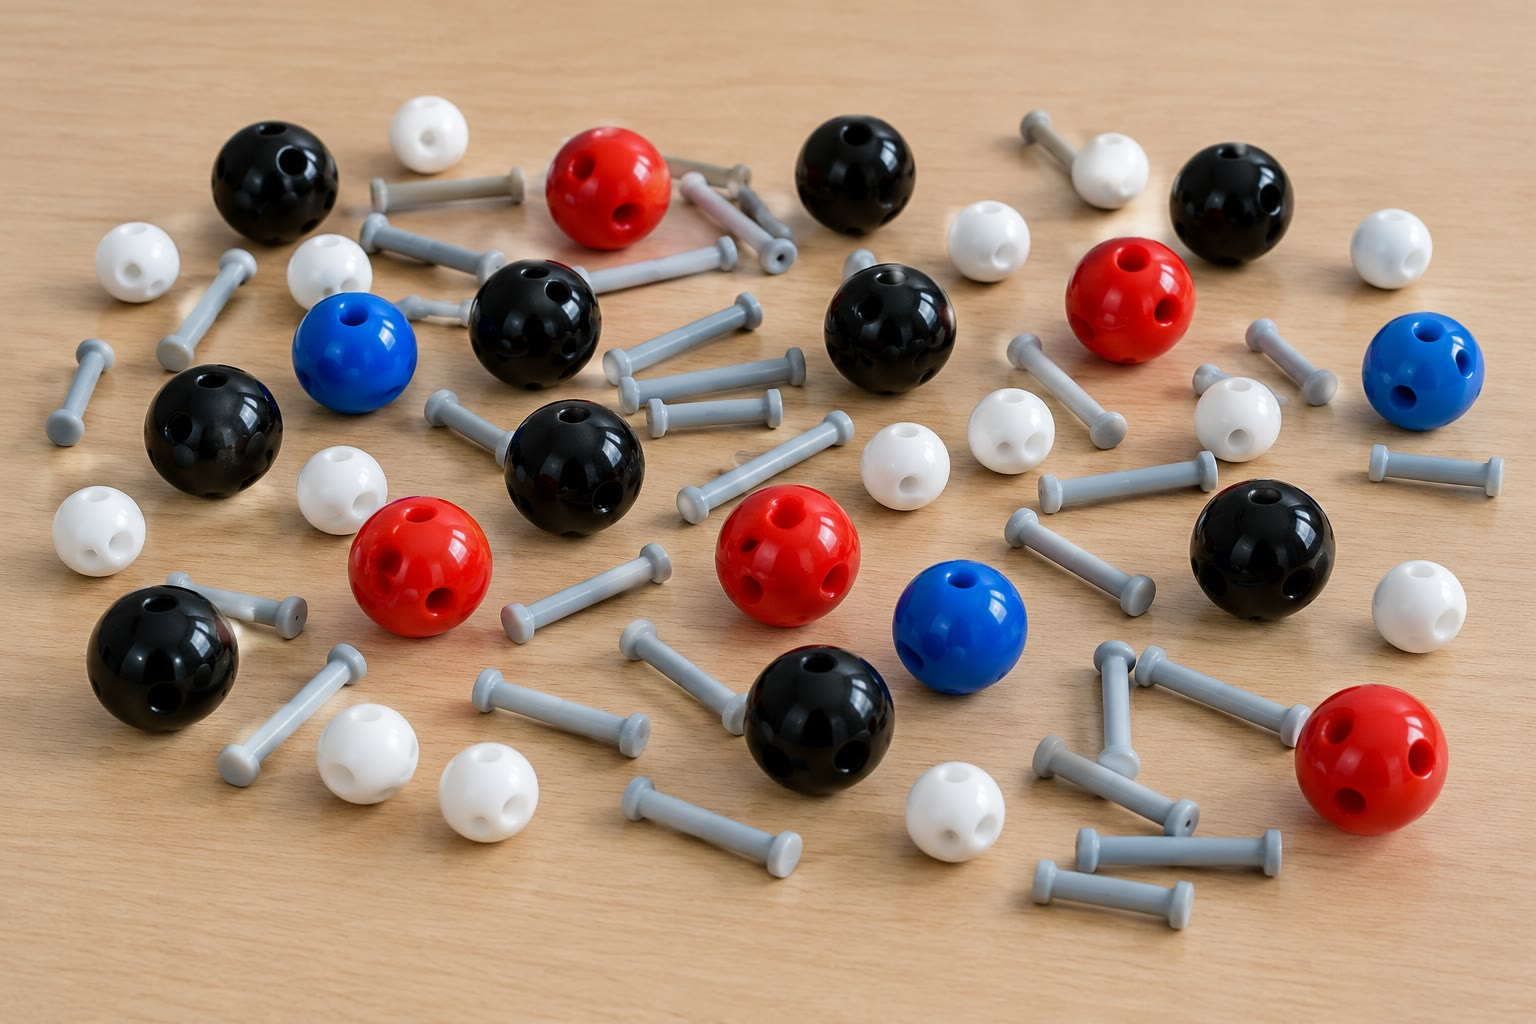
\includegraphics[width=0.5\linewidth]{images/book1/ai/g7-model-kit.jpg}

{\small A molecular model kit: balls for \omterm{def:g7:atoms-and-molecules:atom}{atoms}, with holes for the
sticks that stand for bonds.}
\end{omfigure}

\begin{method}[From a model to a formula]\label{met:g7:atoms-and-molecules:model}
To write the formula of a \omterm{def:g7:atoms-and-molecules:molecule}{molecule} from its model:
\begin{enumerate}
  \item name the \omterm{def:g7:atoms-and-molecules:atom}{atoms} from their colours;
  \item count the balls of each colour;
  \item write the \omterm{def:g7:atoms-and-molecules:symbol}{symbols} with the counts as \omterm{def:g7:atoms-and-molecules:formula}{subscripts}, carbon first,
        then hydrogen, then the other \omterm{def:g7:atoms-and-molecules:atom}{atoms} in alphabetical order of
        their \omterm{def:g7:atoms-and-molecules:symbol}{symbols}.
\end{enumerate}
A black ball joined to four white ones: one carbon, four hydrogen,
\ce{CH4}.
\end{method}

\section{Exercises}

\begin{exercise}[$\star$]\label{exo:g7:atoms-and-molecules:1}
What is an \omterm{def:g7:atoms-and-molecules:atom}{atom}? What is a \omterm{def:g7:atoms-and-molecules:molecule}{molecule}?
\end{exercise}

\begin{exercise}[$\star$]\label{exo:g7:atoms-and-molecules:2}
Give the \omterm{def:g7:atoms-and-molecules:symbol}{symbols} of hydrogen, carbon, nitrogen, oxygen, sodium and
iron.
\end{exercise}

\begin{exercise}[$\star$]\label{exo:g7:atoms-and-molecules:3}
How many \omterm{def:g7:atoms-and-molecules:atom}{atoms} of each kind are there in one \omterm{def:g7:atoms-and-molecules:molecule}{molecule} of carbon
dioxide, \ce{CO2}? How many \omterm{def:g7:atoms-and-molecules:atom}{atoms} in all?
\end{exercise}

\begin{exercise}[$\star$]\label{exo:g7:atoms-and-molecules:4}
Name the \omterm{def:g7:atoms-and-molecules:molecule}{molecules} \ce{H2O}, \ce{O2}, \ce{CH4} and \ce{N2}.
\end{exercise}

\begin{exercise}[$\star$]\label{exo:g7:atoms-and-molecules:5}
A \omterm{def:g7:atoms-and-molecules:molecule}{molecule} of nitrogen dioxide, a brown gas found in polluted \omterm{def:g4:air-a-mixture-of-gases:air}{air}, is
made of one nitrogen \omterm{def:g7:atoms-and-molecules:atom}{atom} and two oxygen \omterm{def:g7:atoms-and-molecules:atom}{atoms}. Write its formula.
\end{exercise}

\begin{exercise}[$\star\star$]\label{exo:g7:atoms-and-molecules:6}
Explain the difference between \ce{O2} and \ce{2O}, and between \ce{CO}
and \ce{Co}.
\end{exercise}

\begin{exercise}[$\star\star$]\label{exo:g7:atoms-and-molecules:7}
How many hydrogen \omterm{def:g7:atoms-and-molecules:atom}{atoms} and how many oxygen \omterm{def:g7:atoms-and-molecules:atom}{atoms} are there in
\ce{3H2O}? In \ce{5O2}?
\end{exercise}

\begin{exercise}[$\star\star$]\label{exo:g7:atoms-and-molecules:8}
A model is made of one black ball joined to two red balls. Name the
\omterm{def:g7:atoms-and-molecules:atom}{atoms}, write the formula, and name the \omterm{def:g7:atoms-and-molecules:molecule}{molecule}.
\end{exercise}

\begin{exercise}[$\star\star$]\label{exo:g7:atoms-and-molecules:9}
In Dalton's table, water is made of one hydrogen \omterm{def:g7:atoms-and-molecules:atom}{atom} and one oxygen
\omterm{def:g7:atoms-and-molecules:atom}{atom}. Write the formula Dalton had in mind, and say how many \omterm{def:g7:atoms-and-molecules:atom}{atoms} his
water \omterm{def:g7:atoms-and-molecules:molecule}{molecule} is missing.
\end{exercise}

\begin{exercise}[$\star\star$]\label{exo:g7:atoms-and-molecules:10}
Is pure water a \omterm{def:g6:pure-substances-and-mixtures:mixture}{mixture}? Is \omterm{def:g4:air-a-mixture-of-gases:air}{air}? Answer by describing the \omterm{def:g7:atoms-and-molecules:molecule}{molecules} each
one contains.
\end{exercise}

\begin{exercise}[$\star\star\star$]\label{exo:g7:atoms-and-molecules:11}
A hydrogen \omterm{def:g7:atoms-and-molecules:atom}{atom} measures about a ten-millionth of a millimetre across.
How many hydrogen \omterm{def:g7:atoms-and-molecules:atom}{atoms}, side by side, would make a line \qty{1}{cm}
long? And a line as long as a football pitch, \qty{100}{m}?
\end{exercise}

\begin{exercise}[$\star\star\star$]\label{exo:g7:atoms-and-molecules:12}
Glucose, the sugar that feeds our cells, has the formula
\ce{C6H12O6}. How many \omterm{def:g7:atoms-and-molecules:atom}{atoms} does one glucose \omterm{def:g7:atoms-and-molecules:molecule}{molecule} contain? What
percentage of them are hydrogen \omterm{def:g7:atoms-and-molecules:atom}{atoms}? What percentage are carbon \omterm{def:g7:atoms-and-molecules:atom}{atoms}?
\end{exercise}

\section{Problem: The Atoms of a Breath}

\begin{problem}[{Weekend problem --- counting the atoms in a breath of
air, before and after it has been in our lungs}]
\label{pb:g7:atoms-and-molecules:1}
% ledger: air:N2, air:O2, air:Ar (78.08 / 20.95 / 0.93 rounded to 78 / 21 / 1),
% breath:O2, breath:CO2, breath:N2 (expired air: 16 / 4 / 78, water vapour removed)
Nitrogen passes through the lungs unchanged, so it makes a good yardstick.
In dry \omterm{def:g4:air-a-mixture-of-gases:air}{air}, for every 78 \omterm{def:g7:atoms-and-molecules:molecule}{molecules} of nitrogen there are about 21 \omterm{def:g7:atoms-and-molecules:molecule}{molecules}
of oxygen and 1 \omterm{def:g7:atoms-and-molecules:atom}{atom} of argon: 100 particles (\omterm{def:g7:atoms-and-molecules:molecule}{molecules} or single \omterm{def:g7:atoms-and-molecules:atom}{atoms}) in
all. In \omterm{def:g4:air-a-mixture-of-gases:air}{air} breathed out, once its water vapour is removed, the same 78
nitrogen \omterm{def:g7:atoms-and-molecules:molecule}{molecules} come with about 16 \omterm{def:g7:atoms-and-molecules:molecule}{molecules} of oxygen, 4 \omterm{def:g7:atoms-and-molecules:molecule}{molecules} of
carbon dioxide and 1 \omterm{def:g7:atoms-and-molecules:atom}{atom} of argon.

\medskip
\noindent\textbf{Part I --- The \omterm{def:g4:air-a-mixture-of-gases:air}{air} we breathe in.}
\begin{enumerate}
  \item Write the formulas of the nitrogen, oxygen and carbon dioxide
        \omterm{def:g7:atoms-and-molecules:molecule}{molecules}, and give the number of \omterm{def:g7:atoms-and-molecules:atom}{atoms} in each.
  \item Argon is counted in \omterm{def:g7:atoms-and-molecules:atom}{atoms}, not in \omterm{def:g7:atoms-and-molecules:molecule}{molecules}. What does this
        tell us about argon?
  \item In these 100 particles of \omterm{def:g4:air-a-mixture-of-gases:air}{air} breathed in, how many nitrogen \omterm{def:g7:atoms-and-molecules:atom}{atoms}
        are there? How many oxygen \omterm{def:g7:atoms-and-molecules:atom}{atoms}?
  \item How many \omterm{def:g7:atoms-and-molecules:atom}{atoms} are there in all in these 100 particles?
  \item What percentage of these \omterm{def:g7:atoms-and-molecules:atom}{atoms} are nitrogen \omterm{def:g7:atoms-and-molecules:atom}{atoms}? Round to the
        nearest whole number.
\end{enumerate}

\medskip
\noindent\textbf{Part II --- The \omterm{def:g4:air-a-mixture-of-gases:air}{air} we breathe out.}
\begin{enumerate}[resume]
  \item In the \omterm{def:g4:air-a-mixture-of-gases:air}{air} breathed out that goes with the same 78 nitrogen
        \omterm{def:g7:atoms-and-molecules:molecule}{molecules}, how many oxygen \omterm{def:g7:atoms-and-molecules:atom}{atoms} are there inside oxygen \omterm{def:g7:atoms-and-molecules:molecule}{molecules}?
        Inside carbon dioxide \omterm{def:g7:atoms-and-molecules:molecule}{molecules}? In all?
  \item Compare with question 3. How many oxygen \omterm{def:g7:atoms-and-molecules:atom}{atoms} are missing? Into
        which \omterm{def:g7:atoms-and-molecules:molecule}{molecule}, made in the body from the hydrogen of food and
        removed here with the water vapour, have they gone?
  \item How many carbon \omterm{def:g7:atoms-and-molecules:atom}{atoms} are there in the \omterm{def:g4:air-a-mixture-of-gases:air}{air} breathed in? In the \omterm{def:g4:air-a-mixture-of-gases:air}{air}
        breathed out?
  \item \omterm{def:g4:air-a-mixture-of-gases:air}{Air} brings no carbon \omterm{def:g7:atoms-and-molecules:atom}{atoms} into the lungs. Where can the carbon
        \omterm{def:g7:atoms-and-molecules:atom}{atoms} of the breath come from? (Think of what the body uses to
        live.)
  \item How many oxygen \omterm{def:g7:atoms-and-molecules:molecule}{molecules} have disappeared, and how many carbon
        dioxide \omterm{def:g7:atoms-and-molecules:molecule}{molecules} have appeared?
\end{enumerate}

\medskip
\noindent\textbf{Part III --- The count.}
\begin{enumerate}[resume]
  \item Describe the ball-and-stick model of each of the four kinds of
        particle in breathed-out \omterm{def:g4:air-a-mixture-of-gases:air}{air}, with the colours of the balls
        (argon is shown as a single pale blue ball).
  \item How many \omterm{def:g7:atoms-and-molecules:atom}{atoms} are there in all in the dried \omterm{def:g4:air-a-mixture-of-gases:air}{air} breathed out?
        By how many \omterm{def:g7:atoms-and-molecules:atom}{atoms} does it exceed the \omterm{def:g4:air-a-mixture-of-gases:air}{air} breathed in? Explain the
        difference with the carbon \omterm{def:g7:atoms-and-molecules:atom}{atoms} gained and the oxygen \omterm{def:g7:atoms-and-molecules:atom}{atoms}
        missing.
\end{enumerate}
\end{problem}
